%.$ xelatex --shell-escape TP1.tex

%path to figures
\newcommand{\figures}{./Figures}

\documentclass[
11pt,
oneside,
french,
singlespacing,
liststotoc,
toctotoc,
headsepline,
]{MastersDoctoralThesis}

\usepackage{mathpazo}
\usepackage{fontspec}
\setmainfont[Ligatures=TeX, Mapping=tex-text]{TeX Gyre Pagella}
\setmonofont{FreeMonoBold}
\usepackage[backend=bibtex, style=authoryear, natbib=true]{biblatex}
\addbibresource{example.bib}
\usepackage[autostyle=true]{csquotes}
\usepackage{enumitem}
\usepackage{float}
\usepackage{amsmath}
\usepackage{minted}
\usepackage{xcolor}

\geometry{
	paper=a4paper,
	inner=2.5cm,
	outer=2.5cm,
	bindingoffset=0.5cm,
	top=1.5cm,
	bottom=1.5cm,
	}

\thesistitle{Autoscope\\Compte rendu final}
\supervisor {}
\examiner{}
\degree{\href{http://www.estei.fr/filiere/informatique-systemes-embarques}{MASTER Systèmes Embarqués}}
\author{Thomas ABGRALL\\Clément AILLOUD\\Thibaud LE DOLEDEC\\\href{https://www.github.com/thomaslepoix}{Thomas LEPOIX}}
\addresses{}
\subject{}
\keywords{}
\university{\href{http://www.estei.fr}{E.S.T.E.I.}}
\department{\href{http://www.estei.fr}{École Supérieure des Technologies Électronique, Informatique, et Infographie}}
\group{\href{http://www.estei.fr/filiere/informatique-systemes-embarques}{Département Systèmes Embarqués}}
\faculty{\href{http://www.estei.fr}{E.S.T.E.I.}}

\AtBeginDocument{
	\hypersetup{pdftitle=\ttitle}
	\hypersetup{pdfauthor=\authorname}
	\hypersetup{pdfkeywords=\keywordnames}
	}

\begin{document}

\mainmatter
\pagestyle{plain}
\usemintedstyle{monokailight}
%bash/Ruby/basemake/
\definecolor{gris}{gray}{0.97}
\definecolor{gris2}{HTML}{282828}
\definecolor{ubuntu}{HTML}{300A24}

\newcommand{\code}[1]{\begin{minted}[
linenos,
breaklines,
breakautoindent,
breakaftersymbolpost,
bgcolor=gris,
fontsize=\scriptsize,
obeytabs,
tabsize=4,
showtabs,
]{#1}}

\newcommand{\codeinline}[2]{\mintinline[fontsize=\footnotesize]{#1}{#2}}


%------------------------------------------------------------------

\begin{titlepage}
\begin{center}

{\href{http://www.estei.fr}{\includegraphics[width=\linewidth]{\figures/estei.png}}}
\vspace*{.06\textheight}
\vspace{1.5cm}\\
\textsc{\Large Projet de MASTER 2}\\[0.5cm]

\HRule \\[0.4cm]
{\huge \bfseries \ttitle\par}\vspace{0.4cm}
\HRule \\[1.5cm]

\large{\emph{Auteurs :}\\
\authorname}

\vspace{4cm}
\degreename\\[1cm]
{\vspace{0.4cm}\scshape\LARGE \univname}\\\deptname\\\groupname\\[1cm]

\vfill

{\large \today}\\[1cm]

\end{center}
\end{titlepage}

%------------------------------------------------------------------

%\begin{acknowledgements}
%\addchaptertocentry{\acknowledgementname} % Add the acknowledgements to the table of contents
%\end{acknowledgements}

\tableofcontents

\pagestyle{thesis}

%chapter Cahier des charges
%chapter Structure 3D
%chapter Hardware
%chapter Middleware
%chapter Software
%chapter Conclusion

\part{Partie de groupe}
\chapter{Hardware}

\section{Rappel sur l'architecture de la carte}

En guise de rappel, ci-dessous un schéma de l'architecture de la carte du télescope.

\begin{figure}[H]
    \centering
    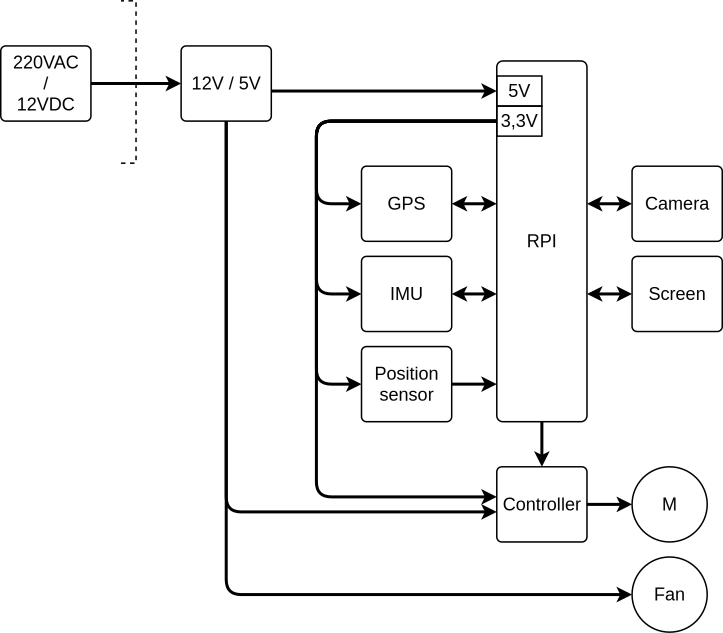
\includegraphics[width=0.7\linewidth]{\figures/sch_hardware.pdf}
    \decoRule
    \caption[
    Schéma structurel de premier niveau du télescope]{
    Schéma structurel de premier niveau du télescope}
    \label{fig:Schéma structurel de premier niveau du télescope}
    \end{figure}

\section{Conception du circuit}

\begin{figure}[H]
    \centering
    \includegraphics[width=1\linewidth]{\figures/kicad_sch2.pdf}
    \decoRule
    \caption[
    Schéma structurel de la carte du télescope]{
    Schéma structurel de la carte du télescope}
    \label{fig:Schéma structurel de la carte du télescope}
    \end{figure}

\vspace{1cm}

Ce schéma ne présente pas de subtilité particulière, la plupart des composants étant des connecteurs.

\vspace{1cm}

L'alimentation est composée de~:
\begin{itemize}[label=$\bullet$]
	\item Un interrupteur d'allumage
	\item Une diode polarisante
	\item Une diode zener protégeant des surtensions
	\item Un fusible protégeant des surintensités
	\item Un convertisseur DC/DC intégré
	\end{itemize}

\vspace{1cm}

L'environnement des boutons poussoirs servant de capteurs de butée aux mouvements du télescope est le suivant~:

\begin{figure}[H]
    \centering
    \includegraphics[width=0.3\linewidth]{\figures/sch_button.pdf}
    \decoRule
    \caption[
    Schéma de l'environnement des capteurs de butée]{
    Schéma de l'environnement des capteurs de butée}
    \label{fig:Schéma de l'environnement des capteurs de butée}
    \end{figure}

\vspace{1cm}

La valeur élevée des résistances de pullup $100k\Omega$ a pour but de réduire au maximum le courant consommé lors de l'appui, à $33\mu A$. Le courant prélevé par l'entrée GPIO de la Raspberry Pi est de l'ordre de $0,5\mu A$.

Les condensateurs de $100nF$ permettent de filtrer les parasites générés par les rebonds propres aux boutons ainsi que les perturbations électromagnétiques.

\section{Contraintes de design}

\subsection{Contraintes électromagnétiques}

La première contrainte vient de la proximité du système électronique de deux moteurs, ceux-ci générant d'importantes perturbations électromagnétiques. Cela peut être particulièrement dérangeant pour le fonctionnement de la centrale inertielle et du GPS.

La solution la plus simple et efficace est de déporter ces deux modules le long de la structure du télescope.

%\vspace{1cm}

\subsection{Contraintes mécaniques}

Ensuite viennent les contraintes mécaniques de l'association de la carte à la Raspberry Pi.

\vspace{1cm}

Tout d'abord, l'emplacement du connecteur et des fixations sont à prendre en compte.

\begin{figure}[H]
    \centering
    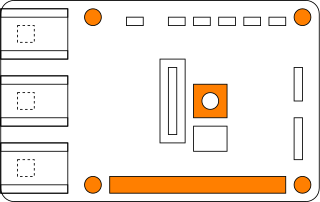
\includegraphics[width=0.5\linewidth]{\figures/sch_hard_1.pdf}
    \decoRule
    \caption[
    Schéma mécanique de la carte vue de dessus]{
    Schéma mécanique de la carte vue de dessus}
    \label{fig:Schéma mécanique de la carte vue de dessus}
    \end{figure}

\vspace{1cm}

Le connecteur d'alimentation, centré sur la carte, est un connecteur cylindrique comme ceux des ordinateurs portables. Le télescope étant amené à tourner sur lui même, ce connecteur devrait permettre le mouvement tout en empêchant le câble d'alimentation de s'emmêler ou de se détériorer.

\begin{figure}[H]
    \centering
    \includegraphics[height=0.3\linewidth]{\figures/photo_supply.jpg}
	\hspace{1cm}
    \includegraphics[height=0.3\linewidth]{\figures/photo_supply.png}
    \decoRule
    \caption[
    Connecteurs d'alimentation utilisés]{
    Connecteurs d'alimentation utilisés}
    \label{fig:Connecteurs d'alimentation utilisés}
    \end{figure}

\vspace{1cm}

Puis concernant la distance entre la carte et la Raspberry Pi, la hauteur des plus hauts éléments de la Raspberry Pi est à prendre en compte. Ainsi que la hauteur de certains condensateurs de la carte, ne pouvant donc être placés n'importe où.

\begin{figure}[H]
    \centering
    
\includegraphics[height=0.23\linewidth]{\figures/sch_hard_2.pdf}
%	\hspace{1cm}
    
\includegraphics[height=0.23\linewidth]{\figures/sch_hard_3.pdf}
    \decoRule
    \caption[
    Schéma mécanique de la carte vue de profil]{
    Schéma mécanique de la carte vue de profil}
    \label{fig:Schéma mécanique de la carte vue de profil}
    \end{figure}

\vspace{1cm}

Il faudra de plus utiliser un connecteur particulièrement haut ($16,13mm$) pour relier la carte à la Raspberry Pi.

\begin{figure}[H]
    \centering
    \includegraphics[width=0.3\linewidth]{\figures/photo_header.png}
    \decoRule
    \caption[
    Type de header utilisé]{
    Type de header utilisé}
    \label{fig:Type de header utilisé}
    \end{figure}

\section{Routage de la carte}

Le routage de la carte n'est pas terminé, voici un aperçu de son avancement actuel~:

\begin{figure}[H]
    \centering
    \includegraphics[width=0.7\linewidth]{\figures/kicad_pcb.png}
    \decoRule
    \caption[
    Aperçu du routage en cours]{
    Aperçu du routage en cours}
    \label{fig:Aperçu du routage en cours}
    \end{figure}


\chapter{Hardware}
\label{chapter2}

\section{Choix des principaux composants}

Les principaux composants électroniques ont étés choisis en premier lieu sur les critères du prix et de la rapidité de mise en œuvre.

\vspace{1cm}

\begin{itemize}[label=$\bullet$]
	\item Le GPS : Le module adafruit-ultimate-gps (MTK3339)
	\item L'IMU : Le module Sarkfun SEN-13762 (MPU9250)
	\item Le convertisseur $12V/5V$ : Le Composant intégré Recom R-78B5.0-2.0 capable de fournir un courant de $2A$.

\section{Procédure de calibration}

Une procédure de calibration du télescope sera sans doute à prévoir à son allumage. Celle-ci ayant pour but de déterminer la direction du nord et la direction verticale.

\vspace{1cm}

À supposer que le télescope soit posé sur une surface proche de l'horizontale, la procédure consisterait~:
\begin{itemize}[label=$\bullet$]
	\item Pour l'azimut, à effectuer une rotation complète pour déterminer la direction dans laquelle le champ magnétique est le plus fort, le nord.
	\item Pour l'élévation, à balayer la plage de mouvement des croissants de la structure en observant les données de l'accéléromètre. La position dans laquelle l'accélération de la 

\chapter{Software}
\label{chapter3}

\section{Support de la caméra}

Pour gérer les différentes configurations matérielles de façon plus "userfriendly", la Raspberry Pi dispose d'un fichier de configuration \codeinline{text}{config.txt} que le $bootloader$ interprétera pour sélectionner les $overlays$ correspondants et composer le $devicetree$ qui convient à l'architecture matérielle utilisée. Celui-ci étant ensuite passé au $kernel$ lors du démarrage.

%\vspace{1cm}

Cette subtilité propre aux Raspberry Pi permet à l'utilisateur de ne pas avoir besoin d'avoir affaire au $devicetree$ quand il s'agit de configuration. Par exemple l'activation du support d'un élément courant sur les Raspberry Pi comme le module Raspicam.

%\vspace{1cm}

le logiciel \codeinline{text}{raspi-config} n'est autre qu'une interface à ce fichier de configuration.

\vspace{1cm}

Pour activer le support matériel de la caméra, il faut ajouter les lignes suivantes à ce fichier~:

%\code{ruby}
\code{bash}
start_x=1
gpu_mem=128
\end{minted}

À travers Yocto, cela passe par l'ajout des lignes ci-dessous au fichier \codeinline{text}{local.conf} et donc à son modèle le fichier \codeinline{text}{meta-autoscope/conf/local.conf.sample} dans la $layer$ dédiée au projet.

\code{ruby}
VIDEO_CAMERA = "1"
GPU_MEM = "128"
\end{minted}

\vspace{1cm}

Quant à l'utilisation de la caméra, il existe des logiciels tels que \codeinline{text}{raspivid} pour filmer ou \codeinline{text}{raspistill} pour prendre des clichés. Tous deux font partie de la suite \codeinline{text}{userland} que l'on ajoute à notre image via la ligne ci-dessous dans le fichier\\\codeinline{text}{meta-autoscope/recipes-autoscope/images/autoscope-console-image.bb}~:

\code{ruby}
IMAGE_INSTALL += "userland"
\end{minted}

À l'usage, la commande suivante permet d'afficher en plein écran le flux vidéo jusqu'à ce qu'on le stoppe~:

\code{bash}
~$ raspivid -t 0
\end{minted}

\section{Étude de l'embarcation de Stellarium}

Une première évaluation de la faisabilité de l'embarcation de Stellarium sur la Raspberry Pi a été de l'installer via le gestionnaire de paquet sur une Raspberry Pi dotée de Raspbian.

\code{bash}
~$ sudo apt-get install stellarium
\end{minted}

\vspace{1cm}

Avec le compositeur graphique logiciel, Stellarium est totalement inutilisable. Cependant il est possible d'activer le compositeur graphique matériel. Pour cela il faut activer l'option \codeinline{text}{Advanced Options -> GL Driver} dans le menu \codeinline{text}{raspi-config}.

La différence de rendu peut être observée avec l'outil \codeinline{text}{glxgears} prévu à cet effet. Celui-ci s'installe par la ligne suivante~:

\code{bash}
~$ sudo apt-get install mesa-utils
\end{minted}

\begin{figure}[H]
    \centering
    \includegraphics[width=0.3\linewidth]{\figures/photo_glxgears.png}
    \decoRule
    \caption[
    Captures d'écran de glxgears]{
    Captures d'écran de glxgears}
    \label{fig:Captures d'écran de glxgears}
    \end{figure}

\vspace{1cm}

Le résultat est alors meilleur, Stellarium est utilisable bien qu'il lui arrive de planter lorsque l'on fait un déplacement trop brusque dans le ciel.

\vspace{1cm}

Il existe une version mobile de Stellarium disponible notament pour Android et iOS qui est une version allélégée et optimisée pour l'usage sur un smartphone.

Ses sources sont disponibles à l'adresse suivante~:\\\url{https://noctua-software.com/stellarium-mobile}

\vspace{1cm}

Il semble que cette version puisse fonctionner telle quelle sur Linux. À l'heure actuelle nous n'avons pas réussi à compiler Stellarium mobile pour un problème de dépendance à une librairie (Qt5Declarative, faisant partie du paquet qtdeclarative5-dev) qui n'existe plus dans les versions récentes de Qt, ultérieures à la version Qt5.6 pour être précis.

Le problème pourrait sans doute être résolu en récupérant ladite librairie dans les dépots d'une distribution plus ancienne, Ubuntu Xenial (Qt5.5.1) ou Trusty (Qt5.2.1) par exemple.


\chapter{Organisation prévisionnelle}
\label{chapter4}

Me concernant, pour le prochain cycle de travail le plus urgent est d'étudier l'aspect hardware du télescope et de produire la carte qui accueillera les différents périphériques de la Raspberry Pi.

\vspace{1cm}

Ensuite ma contribution pourrait être la plus utile dans l'intégration au système d'exploitation des différents éléments qui le composent, comme le logiciel principal de l'Autoscope ou les logiciels Siril et éventuellement Stellarium. Ou bien dans les choix ergonomiques préalables au développement de l'interface utilisateur.

\chapter{Stellarium}

Ce chapitre n'a pas vocation à expliquer comment fonctionne le plugin de Stellarium développé par Thibaud LE DOLEDEC mais la procédure à suivre pour pouvoir utiliser ce plugin.

\vspace{1cm}

Ajouter un plugin à ce logiciel nécessite de modifier son code source et donc de recompiler l'intégralité du logiciel.

\section{Installation depuis les sources}

Installation des dépendances (sur une distribution de type Debian/Ubuntu)~:

\code{text}
~ $
    sudo apt-get install build-essential cmake zlib1g-dev libgl1-mesa-dev gcc g++
    sudo apt-get install graphviz doxygen gettext git
\end{minted}

\vspace{1cm}

Installation des dépendances Qt~:

\code{text}
~ $
    mkdir DEV/
    cd DEV/
    wget http://download.qt.io/archive/qt/5.5/5.5.0/qt-opensource-linux-x64-5.5.0-2.run
    chmod +x qt-opensource-linux-x64-5.5.0-2.run
    ./qt-opensource-linux-x64-5.5.0-2.run
    #enter a shitty email address (e.g. qt.qt@yopmail.com)
    #install in /opt/Qt5.5.0/

    git clone https://github.com/qt/qtftp
    cd qtftp/
    /opt/Qt5.5.0/5.5/gcc_64/bin/syncqt.pl -version 5.5.0
    /opt/Qt5.5.0/5.5/gcc_64/bin/qmake
    make
    sudo make install
\end{minted}

\vspace{1cm}

Téléchargement des sources de Stellarium et du plugin Autoscope~:

\code{text}
~/DEV $
    wget https://github.com/Stellarium/stellarium/releases/download/v0.19.0/ stellarium-0.19.0.tar.gz
    tar -xzf stellarium-0.19.0.tar.gz
    cd stellarium-0.19.0/plugins/
    git clone https://github.com/thibaudledo/Autoscope-Stellarium-plugin.git plugins/Autoscope
\end{minted}

\vspace{1cm}

Activation du plugin. Cela peut être fait en modifiant manuellement les sources de Stellarium ou en appliquant un patch de la modification fourni avec les sources du plugin~:

\code{text}
~/DEV/Stellarium-0.19.0 $
    git init
    git add CMakeLists.txt src/core/StelApp.cpp
    git apply plugins/Autoscope/0001-enable-autoscope-plugin.patch

    ### OR APPEND MANUALLY ###
    line 369 : CMakeLists.txt
        ADD_PLUGIN(Autoscope 1)
    line 94 : src/core/StelApp.cpp
        #ifdef USE_STATIC_PLUGIN_AUTOSCOPE
        Q_IMPORT_PLUGIN(AutoscopeStelPluginInterface)
        #endif
\end{minted}

\vspace{1cm}

Export de l'emplacement de Qt~:

\code{text}
    export QTDIR=/opt/Qt5.5.0/5.5/gcc_64
    export PATH=/opt/Qt5.5.0/5.5/gcc_64/bin:${PATH}
    export LD_LIBRARY_PATH=${QTPATH}/lib:${LD_LIBRARY_PATH}
\end{minted}

\vspace{1cm}

Compilation de Stellarium~:

\code{text}
~/DEV/Stellarium-0.19.0 $
    mkdir -p builds/unix/
    cd builds/unix/
    cmake -DCMAKE_BUILD_MODE=Release -DCMAKE_INSTALL_PREFIX=/opt/stellarium ../../
    make -j4
\end{minted}

\vspace{1cm}

Installation de Stellarium~:

\code{text}
~/DEV/Stellarium-0.19.0/builds/unix $
    sudo make install
\end{minted}

\section{Création d'un paquet binaire}

Après la compilation il est possible d'installer le logiciel mais il est aussi possible de créer des paquets permettant de le distribuer. L'on peut créer~:
\begin{itemize}[label=$\bullet$]
	\item Un paquet contenant le code source de Stellarium et du plugin, prêt à être compilé.
	\item Un paquet contenant le logiciel compilé, à installer manuellement.
	\item Un paquet \codeinline{text}{.deb} contenant le logiciel compilé et destiné au logiciel de gestion de paquets des distributions GNU/Linux de la famille Debian.
	\item Un paquet \codeinline{text}{.rmp} contenant le logiciel compilé et destiné au logiciel de gestion de paquets des distributions GNU/Linux de la famille Red Hat.
	\end{itemize}

\code{text}
~/DEV/Stellarium-0.19.0/builds/unix $
    make package_source
    make package
    cpack -G DEB
    cpack -G RPM
\end{minted}

\section{Installation manuelle d'un paquet binaire}

L'on choisit d'installer le logiciel dans le dossier \codeinline{text}{/opt} plutôt que \codeinline{text}{/usr/local} dans le but de l'isoler un peu et de permettre un développement moins risqué ainsi que la cohabitation d'une version Autoscope de Stellarium installée manuellement et d'une version classique installée depuis le gestionnaire de paquets.

Dans le dossier \codeinline{text}{/opt}, chaque logiciel installé dispose d'un dossier lui étant propre, tandis que dans \codeinline{text}{/usr} et \codeinline{text}{/usr/local}, l'arborescence est partagée à tous les logiciels (les binaires avec les binaires, les sources avec les sources, les icônes avec les icônes, etc.). Le dossier \codeinline{text}{/opt} n'est généralement pas utilisé par les gestionnaires de paquets.

\vspace{1cm}

Un paquet binaire est disponible sur le dépôt du projet, à l'adresse suivante~:

{\href{https://github.com/thibaudledo/Autoscope/releases/tag/alpha}{\codeinline{text}{https://github.com/thibaudledo/Autoscope/releases/tag/alpha}}}

\code{text}
/opt #
    wget https://github.com/thibaudledo/Autoscope/releases/download/alpha/ Stellarium-0.19.0-Linux.tar.gz
    tar -xzf Stellarium-0.19.0-Linux.tar.gz
\end{minted}

\section{Lancement de Stellarium}

La commande suivante peut être utilisée pour créer un raccourcis dans un dock, un tableau de bord ou un menu~:

\code{text}
~ $
    /opt/Stellarium-0.19.0-Linux/bin/stellarium
\end{minted}


\chapter{Travail effectué par Thibaud LE DOLEDEC et Clément AILLOUD}

\section{Driver de la centrale inertielle (IMU)}

Clément AILLOUD a développé un driver Linux pour la centrale inertielle en utilisant le framework \codeinline{text}{iio}. Celui-ci supporte actuellement le gyroscope et l'accéléromètre mais pas le magnétomètre. Il est compatible avec les bus I2C et SPI. Sur l'Autoscope, le bus I2C sera utilisé.

Un patch du device tree permettant le support du driver est également fourni.

\vspace{1cm}

Le driver a été intégré au système d'exploitation du télescope. \codeinline{text}{iio} permet d'accéder aux données issues de l'IMU via le dossier suivant~:

\code{text}
root@autoscope ~ #
    ls /sys/bus/iio/devices/iio:device0/
        dev               in_accel_y_raw    in_anglvel_x_raw  in_temp_input  power
        in_accel_scale    in_accel_z_raw    in_anglvel_y_raw  name           subsystem
        in_accel_x_raw    in_anglvel_scale  in_anglvel_z_raw  of_node        uevent

    cat /sys/bus/iio/devices/iio:device0/name
        mpu9250-i2c
\end{minted}

\section{Interface utilisateur (Plugin de Stellarium)}

Le logiciel Stellarium offre la possibilité de développer des plugins aux fonctionnalités diverses. Nous avons décidé d'utiliser un plugin pour faire de Stellarium l'élément principal de l'interface utilisateur du télescope.

\vspace{1cm}

Thibaud LE DOLEDEC a développé un plugin de Stellarium permettant les actions suivantes~:
\begin{itemize}[label=$\bullet$]
	\item Rechercher un astre et le suivre tant à l'écran qu'avec le télescope (par l'envoi régulier de coordonnées spatiales à celui-ci).
	\item Demander au télescope ses coordonnées de position et de visée et afficher la vue du ciel simulé correspondante.
	\item Ordonner au télescope de prendre une photo. Il existe une interface destinée à configurer les paramètres de la caméra (temps d'exposition, etc.).
	\item Se connecter au serveur FTP du télescope pour récupérer les clichés du ciel.
	\item Afficher un aperçu de ce que voit le télescope à l'instant présent (retransmission d'un flux vidéo). Un espace actuellement matérialisé par un rectangle gris est destiné à cela.
	\end{itemize}

\vspace{1cm}

\begin{figure}[H]
    \centering
    \includegraphics[width=0.9\linewidth]{\figures/photo_stellarium_3.png}
    \includegraphics[width=0.9\linewidth]{\figures/photo_stellarium_4.png}
    \decoRule
    \caption[
    Aperçu de l'interface du plugin de Stellarium]{
    Aperçu de l'interface du plugin de Stellarium}
    \label{fig:Aperçu de l'interface du plugin de Stellarium}
    \end{figure}

\vspace{1cm}

Le plugin fonctionne correctement, bien que certains éléments soient sûrement à retravailler lors du développement du logiciel principal du télescope.

La gestion de la communication FTP repose sur l'utilisation d'une librairie dépréciée \codeinline{text}{qtftp} qui a semblé poser problème lors des essais de déploiement du travail réalisé par Thibaud. L'idéal serait de se passer de cette librairie.

\vspace{1cm}

Thibaud et Clément ont rédigé un document disponible à l'adresse suivante qui explique la procédure à suivre pour développer un plugin de Stellarium.

{\href{https://github.com/thibaudledo/Autoscope/blob/latex/Tutoriel_Stellarium.pdf}{\codeinline{text}{https://github.com/thibaudledo/Autoscope/blob/latex/Tutoriel_Stellarium.pdf}}}

\chapter{Travail restant à faire}

Ce chapitre existe dans le but de récapituler le travail restant à faire sur le projet de façon un minimum exhaustive.

\section{Structure du télescope}

La plupart des pièces du télescope vierge de toute modification a été imprimée, quelques parties assemblées. Le travail restant à faire est conséquent et consiste en la modification du design du télescope en vue d'y intégrer~:
\begin{itemize}[label=$\bullet$]
	\item La carte électronique et la Raspberry-pi, face vers le sol, sous le miroir primaire.
	\item Les modules GPS et IMU, placés le long de la structure du télescope. L'interprétation des données émises par l'IMU dépendra de son positionnement.
	\item Les moteurs d'azimut et d'élévation ainsi que leurs courroies et tringles. Les roues crantées à fixer sur l'axe des moteurs n'ont pas été choisies. Leur diamètre reste à déterminer.
	\item Les boutons poussoirs, capteurs de fin de course des mouvements engendrés par les moteur. Leur position devra être déterminée avec précision.
	\item Tout le dispositif maintenant l'oculaire, le moteur permettant de l'actionner, les capteurs de fin de course associés (le mouvement de l'oculaire s'étend sur environ un quart de tour), ainsi que le module caméra. Ce dispositif devra être conçu avec le plus grand soin et la plus grande attention afin de permettre un réglage fin du télescope et d'obtenir une image nette. Il est conseillé de se renseigner la procédure de $collimation$ des télescopes avant de se lancer dans la conception.
	\end{itemize}

\section{Hardware}

Il reste uniquement à faire la connectique des éléments déportés de la carte électronique.

Un ventilateur de refroidissement du miroir peut aussi être choisi, nous ne nous sommes pas renseignés sur l'utilité avérée ou non de cet élément.

\section{Système d'exploitation}

\begin{itemize}[label=$\bullet$]
	\item Sécurisation du système par la mise en place d'un pare feu avec \codeinline{text}{iptables} (et donc l'étude des ports utilisés, ainsi que le choix d'un port ne posant aucun conflit pour le transfert vidéo et la communication avec le plugin Stellarium), une gestion plus fine des droits de chaque utilisateur Linux, etc. L'abandon de FTP au profit de SFTP comme protocole de transfert d'images serait souhaitable (\codeinline{text}{openSSH} déjà utilisé comme serveur SSH permet cela).
	\item La mise en place d'un système de mise à jour de l'OS. \codeinline{text}{SWUpdate} semble être une solution plus intéressante que \codeinline{text}{Mender} puisque nettement plus souple et configurable, tant dans la façon de mettre à jour le système que dans la façon de déclencher la mise à jour. Dans tous les cas, ces systèmes de mise à jour nécessitent d'utiliser un bootloader en plus du firmware du GPU de la Raspberry-Pi, or l'overlay du device tree \codeinline{text}{pi3-disable-bt} (nécessaire pour la communication avec le GPS) semble être incompatible avec U-Boot. Une tentative de transformer l'overlay en patch n'a pas résolu le problème, les investigations n'ont pas été poussées davantage.
	\item L'optimisation de l'OS. Plusieurs choses peuvent être optimisées, la mémoire occupée, le temps de boot (qui peut être optimisé à plusieurs niveau, les plus faciles à travailler étant le niveau applicatif et le niveau de processus d'initialisation, ensuite viennent Linux et bootloader). Sur Yocto, le fichier \codeinline{text}{meta-autoscope/conf/distro/autoscope.conf} permet de se délester du support d'éléments inutilisés. Le lien suivant est une documentation intéressante~:\\\url{https://embexus.com/2017/05/16/embedded-linux-fast-boot-techniques/}
	\end{itemize}

\section{Support de la caméra}

Il faut évaluer les possibilités de paramétrage de la capture photo que permettent les logiciels \codeinline{text}{raspistill}, \codeinline{text}{raspiyuv}, etc. Peut être cela est suffisant, peut être existe il une librairie de plus bas niveau utilisable dans un programme C/C++, peut être sera il nécessaire d'en développer une. Il semble peu probable qu'il faille modifier le driver de la caméra.

\section{Transfert du flux vidéo sur le réseau}

La communauté Raspberry-Pi fournit une librairie Python de contrôle de la caméra, il semble qu'elle permette un transfert sur le réseau du flux vidéo sans latence excessive. La recette Yocto pour intégrer ladite librairie a été écrite mais pas celle permettant l'ajout de toutes celles qu'elle même utilise.

Il serait préférable de trouver une librairie équivalente en C/C++, ou à défaut de l'écrire.

\vspace{1cm}

Il n'a pas été déterminé s'il est plus pertinent d'intégrer le logiciel de transmission du flux vidéo au logiciel principal du télescope ou s'il est plus pertinent d'en faire un autre logiciel.

Le serveur vidéo devra probablement s'interrompre le temps que le télescope utilise la caméra pour prendre une photo ponctuelle. Dans le cas où il serait un logiciel distinct du logiciel principal, les signaux seraient sûrement pour ce dernier un moyen de contrôle suffisant. Par exemple \codeinline{text}{SIGSTOP} et \codeinline{text}{SIGCONT} s'il suffit de mettre le serveur en pause, \codeinline{text}{SIGUSR1} et \codeinline{text}{SIGUSR2} si le serveur doit effectuer des actions de connexion/déconnexion au client ainsi qu'à la caméra.

\section{Daemon du GPS}

Le daemon du GPS n'a pas été testé dans un environnement où la connexion est suffisamment bonne pour que le GPS parvienne à calculer sa position géographique. Il suffit probablement de l'emmener à l'extérieur. Ce test permettrait de valider définitivement le fonctionnement du daemon ainsi que du GPS.

Une meilleure gestion des cas d'erreurs dans le code du daemon serait la bienvenue.

\section{Driver des contrôleurs moteur}

Le cœur du driver des contrôleurs moteur fonctionne. L'organe de communication avec le logiciel principal du télescope est le dernier à être en cours de développement bien que proche d'un état satisfaisant.

Quelques éléments légers resteront a modifier. Une phase de refactoring du code sera également nécessaire.

\section{Driver de la centrale inertielle (IMU)}

\begin{itemize}[label=$\bullet$]
	\item Le plus important du travail a été réalisé puisque le driver existe et supporte le gyroscope et l'accéléromètre de la centrale inertielle. Il reste à programmer le support du magnétomètre.
	\item Davantage de documentation sur le fonctionnement du driver serait également bienvenue.
	\item Enfin, une série de tests reste à concevoir et à mettre en œuvre pour valider le fonctionnement du driver.
	\end{itemize}

\section{Plugin de Stellarium}

\begin{itemize}[label=$\bullet$]
	\item La librairie FTP utilisée \codeinline{text}{qftp} pose problème et est dépréciée, il faudrait se passer de son utilisation. Il serait judicieux d'en profiter pour migrer vers SFTP, plus sécurisé.
	\item Une partie du code sera probablement à retravailler conjointement au développement du logiciel principal du télescope, ainsi que du serveur vidéo.
	\end{itemize}

\section{Logiciel principal du télescope (Autoscope-core)}

\begin{itemize}[label=$\bullet$]
	\item Intégration dans un programme unique des fragments d'interface avec les différents organes logiciels du télescope (drivers moteurs et IMU, daemon GPS, plugin Stellarium, etc). Ces fragments se trouvent sur la branche {\href{https://github.com/thibaudledo/Autoscope/tree/master}{\codeinline{text}{master} du dépôt git principal}} et sont voués à disparaître une fois cette tâche effectuée.
	\item Développement de l'algorithme de déplacement du télescope. Celui-ci va dépendre des données qu'il est possible d'obtenir de la centrale inertielle, des possibilités du driver des contrôleurs moteur, ainsi que de la structure du télescope et la façon dont sera intégrée le hardware.
	\end{itemize}


\part{Thomas LEPOIX}
%\chapter{Hardware}

\section{Rappel sur l'architecture de la carte}

En guise de rappel, ci-dessous un schéma de l'architecture de la carte du télescope.

\begin{figure}[H]
    \centering
    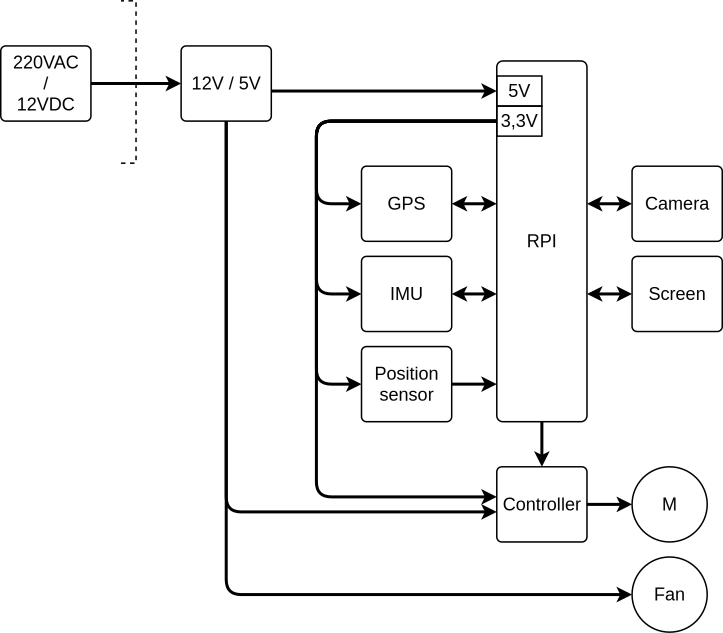
\includegraphics[width=0.7\linewidth]{\figures/sch_hardware.pdf}
    \decoRule
    \caption[
    Schéma structurel de premier niveau du télescope]{
    Schéma structurel de premier niveau du télescope}
    \label{fig:Schéma structurel de premier niveau du télescope}
    \end{figure}

\section{Conception du circuit}

\begin{figure}[H]
    \centering
    \includegraphics[width=1\linewidth]{\figures/kicad_sch2.pdf}
    \decoRule
    \caption[
    Schéma structurel de la carte du télescope]{
    Schéma structurel de la carte du télescope}
    \label{fig:Schéma structurel de la carte du télescope}
    \end{figure}

\vspace{1cm}

Ce schéma ne présente pas de subtilité particulière, la plupart des composants étant des connecteurs.

\vspace{1cm}

L'alimentation est composée de~:
\begin{itemize}[label=$\bullet$]
	\item Un interrupteur d'allumage
	\item Une diode polarisante
	\item Une diode zener protégeant des surtensions
	\item Un fusible protégeant des surintensités
	\item Un convertisseur DC/DC intégré
	\end{itemize}

\vspace{1cm}

L'environnement des boutons poussoirs servant de capteurs de butée aux mouvements du télescope est le suivant~:

\begin{figure}[H]
    \centering
    \includegraphics[width=0.3\linewidth]{\figures/sch_button.pdf}
    \decoRule
    \caption[
    Schéma de l'environnement des capteurs de butée]{
    Schéma de l'environnement des capteurs de butée}
    \label{fig:Schéma de l'environnement des capteurs de butée}
    \end{figure}

\vspace{1cm}

La valeur élevée des résistances de pullup $100k\Omega$ a pour but de réduire au maximum le courant consommé lors de l'appui, à $33\mu A$. Le courant prélevé par l'entrée GPIO de la Raspberry Pi est de l'ordre de $0,5\mu A$.

Les condensateurs de $100nF$ permettent de filtrer les parasites générés par les rebonds propres aux boutons ainsi que les perturbations électromagnétiques.

\section{Contraintes de design}

\subsection{Contraintes électromagnétiques}

La première contrainte vient de la proximité du système électronique de deux moteurs, ceux-ci générant d'importantes perturbations électromagnétiques. Cela peut être particulièrement dérangeant pour le fonctionnement de la centrale inertielle et du GPS.

La solution la plus simple et efficace est de déporter ces deux modules le long de la structure du télescope.

%\vspace{1cm}

\subsection{Contraintes mécaniques}

Ensuite viennent les contraintes mécaniques de l'association de la carte à la Raspberry Pi.

\vspace{1cm}

Tout d'abord, l'emplacement du connecteur et des fixations sont à prendre en compte.

\begin{figure}[H]
    \centering
    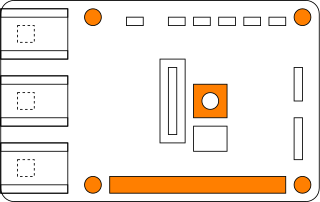
\includegraphics[width=0.5\linewidth]{\figures/sch_hard_1.pdf}
    \decoRule
    \caption[
    Schéma mécanique de la carte vue de dessus]{
    Schéma mécanique de la carte vue de dessus}
    \label{fig:Schéma mécanique de la carte vue de dessus}
    \end{figure}

\vspace{1cm}

Le connecteur d'alimentation, centré sur la carte, est un connecteur cylindrique comme ceux des ordinateurs portables. Le télescope étant amené à tourner sur lui même, ce connecteur devrait permettre le mouvement tout en empêchant le câble d'alimentation de s'emmêler ou de se détériorer.

\begin{figure}[H]
    \centering
    \includegraphics[height=0.3\linewidth]{\figures/photo_supply.jpg}
	\hspace{1cm}
    \includegraphics[height=0.3\linewidth]{\figures/photo_supply.png}
    \decoRule
    \caption[
    Connecteurs d'alimentation utilisés]{
    Connecteurs d'alimentation utilisés}
    \label{fig:Connecteurs d'alimentation utilisés}
    \end{figure}

\vspace{1cm}

Puis concernant la distance entre la carte et la Raspberry Pi, la hauteur des plus hauts éléments de la Raspberry Pi est à prendre en compte. Ainsi que la hauteur de certains condensateurs de la carte, ne pouvant donc être placés n'importe où.

\begin{figure}[H]
    \centering
    
\includegraphics[height=0.23\linewidth]{\figures/sch_hard_2.pdf}
%	\hspace{1cm}
    
\includegraphics[height=0.23\linewidth]{\figures/sch_hard_3.pdf}
    \decoRule
    \caption[
    Schéma mécanique de la carte vue de profil]{
    Schéma mécanique de la carte vue de profil}
    \label{fig:Schéma mécanique de la carte vue de profil}
    \end{figure}

\vspace{1cm}

Il faudra de plus utiliser un connecteur particulièrement haut ($16,13mm$) pour relier la carte à la Raspberry Pi.

\begin{figure}[H]
    \centering
    \includegraphics[width=0.3\linewidth]{\figures/photo_header.png}
    \decoRule
    \caption[
    Type de header utilisé]{
    Type de header utilisé}
    \label{fig:Type de header utilisé}
    \end{figure}

\section{Routage de la carte}

Le routage de la carte n'est pas terminé, voici un aperçu de son avancement actuel~:

\begin{figure}[H]
    \centering
    \includegraphics[width=0.7\linewidth]{\figures/kicad_pcb.png}
    \decoRule
    \caption[
    Aperçu du routage en cours]{
    Aperçu du routage en cours}
    \label{fig:Aperçu du routage en cours}
    \end{figure}


\chapter{Hardware}
\label{chapter2}

\section{Choix des principaux composants}

Les principaux composants électroniques ont étés choisis en premier lieu sur les critères du prix et de la rapidité de mise en œuvre.

\vspace{1cm}

\begin{itemize}[label=$\bullet$]
	\item Le GPS : Le module adafruit-ultimate-gps (MTK3339)
	\item L'IMU : Le module Sarkfun SEN-13762 (MPU9250)
	\item Le convertisseur $12V/5V$ : Le Composant intégré Recom R-78B5.0-2.0 capable de fournir un courant de $2A$.

\section{Procédure de calibration}

Une procédure de calibration du télescope sera sans doute à prévoir à son allumage. Celle-ci ayant pour but de déterminer la direction du nord et la direction verticale.

\vspace{1cm}

À supposer que le télescope soit posé sur une surface proche de l'horizontale, la procédure consisterait~:
\begin{itemize}[label=$\bullet$]
	\item Pour l'azimut, à effectuer une rotation complète pour déterminer la direction dans laquelle le champ magnétique est le plus fort, le nord.
	\item Pour l'élévation, à balayer la plage de mouvement des croissants de la structure en observant les données de l'accéléromètre. La position dans laquelle l'accélération de la 

\chapter{Software}
\label{chapter3}

\section{Support de la caméra}

Pour gérer les différentes configurations matérielles de façon plus "userfriendly", la Raspberry Pi dispose d'un fichier de configuration \codeinline{text}{config.txt} que le $bootloader$ interprétera pour sélectionner les $overlays$ correspondants et composer le $devicetree$ qui convient à l'architecture matérielle utilisée. Celui-ci étant ensuite passé au $kernel$ lors du démarrage.

%\vspace{1cm}

Cette subtilité propre aux Raspberry Pi permet à l'utilisateur de ne pas avoir besoin d'avoir affaire au $devicetree$ quand il s'agit de configuration. Par exemple l'activation du support d'un élément courant sur les Raspberry Pi comme le module Raspicam.

%\vspace{1cm}

le logiciel \codeinline{text}{raspi-config} n'est autre qu'une interface à ce fichier de configuration.

\vspace{1cm}

Pour activer le support matériel de la caméra, il faut ajouter les lignes suivantes à ce fichier~:

%\code{ruby}
\code{bash}
start_x=1
gpu_mem=128
\end{minted}

À travers Yocto, cela passe par l'ajout des lignes ci-dessous au fichier \codeinline{text}{local.conf} et donc à son modèle le fichier \codeinline{text}{meta-autoscope/conf/local.conf.sample} dans la $layer$ dédiée au projet.

\code{ruby}
VIDEO_CAMERA = "1"
GPU_MEM = "128"
\end{minted}

\vspace{1cm}

Quant à l'utilisation de la caméra, il existe des logiciels tels que \codeinline{text}{raspivid} pour filmer ou \codeinline{text}{raspistill} pour prendre des clichés. Tous deux font partie de la suite \codeinline{text}{userland} que l'on ajoute à notre image via la ligne ci-dessous dans le fichier\\\codeinline{text}{meta-autoscope/recipes-autoscope/images/autoscope-console-image.bb}~:

\code{ruby}
IMAGE_INSTALL += "userland"
\end{minted}

À l'usage, la commande suivante permet d'afficher en plein écran le flux vidéo jusqu'à ce qu'on le stoppe~:

\code{bash}
~$ raspivid -t 0
\end{minted}

\section{Étude de l'embarcation de Stellarium}

Une première évaluation de la faisabilité de l'embarcation de Stellarium sur la Raspberry Pi a été de l'installer via le gestionnaire de paquet sur une Raspberry Pi dotée de Raspbian.

\code{bash}
~$ sudo apt-get install stellarium
\end{minted}

\vspace{1cm}

Avec le compositeur graphique logiciel, Stellarium est totalement inutilisable. Cependant il est possible d'activer le compositeur graphique matériel. Pour cela il faut activer l'option \codeinline{text}{Advanced Options -> GL Driver} dans le menu \codeinline{text}{raspi-config}.

La différence de rendu peut être observée avec l'outil \codeinline{text}{glxgears} prévu à cet effet. Celui-ci s'installe par la ligne suivante~:

\code{bash}
~$ sudo apt-get install mesa-utils
\end{minted}

\begin{figure}[H]
    \centering
    \includegraphics[width=0.3\linewidth]{\figures/photo_glxgears.png}
    \decoRule
    \caption[
    Captures d'écran de glxgears]{
    Captures d'écran de glxgears}
    \label{fig:Captures d'écran de glxgears}
    \end{figure}

\vspace{1cm}

Le résultat est alors meilleur, Stellarium est utilisable bien qu'il lui arrive de planter lorsque l'on fait un déplacement trop brusque dans le ciel.

\vspace{1cm}

Il existe une version mobile de Stellarium disponible notament pour Android et iOS qui est une version allélégée et optimisée pour l'usage sur un smartphone.

Ses sources sont disponibles à l'adresse suivante~:\\\url{https://noctua-software.com/stellarium-mobile}

\vspace{1cm}

Il semble que cette version puisse fonctionner telle quelle sur Linux. À l'heure actuelle nous n'avons pas réussi à compiler Stellarium mobile pour un problème de dépendance à une librairie (Qt5Declarative, faisant partie du paquet qtdeclarative5-dev) qui n'existe plus dans les versions récentes de Qt, ultérieures à la version Qt5.6 pour être précis.

Le problème pourrait sans doute être résolu en récupérant ladite librairie dans les dépots d'une distribution plus ancienne, Ubuntu Xenial (Qt5.5.1) ou Trusty (Qt5.2.1) par exemple.


\chapter{Organisation prévisionnelle}
\label{chapter4}

Me concernant, pour le prochain cycle de travail le plus urgent est d'étudier l'aspect hardware du télescope et de produire la carte qui accueillera les différents périphériques de la Raspberry Pi.

\vspace{1cm}

Ensuite ma contribution pourrait être la plus utile dans l'intégration au système d'exploitation des différents éléments qui le composent, comme le logiciel principal de l'Autoscope ou les logiciels Siril et éventuellement Stellarium. Ou bien dans les choix ergonomiques préalables au développement de l'interface utilisateur.

\chapter{Stellarium}

Ce chapitre n'a pas vocation à expliquer comment fonctionne le plugin de Stellarium développé par Thibaud LE DOLEDEC mais la procédure à suivre pour pouvoir utiliser ce plugin.

\vspace{1cm}

Ajouter un plugin à ce logiciel nécessite de modifier son code source et donc de recompiler l'intégralité du logiciel.

\section{Installation depuis les sources}

Installation des dépendances (sur une distribution de type Debian/Ubuntu)~:

\code{text}
~ $
    sudo apt-get install build-essential cmake zlib1g-dev libgl1-mesa-dev gcc g++
    sudo apt-get install graphviz doxygen gettext git
\end{minted}

\vspace{1cm}

Installation des dépendances Qt~:

\code{text}
~ $
    mkdir DEV/
    cd DEV/
    wget http://download.qt.io/archive/qt/5.5/5.5.0/qt-opensource-linux-x64-5.5.0-2.run
    chmod +x qt-opensource-linux-x64-5.5.0-2.run
    ./qt-opensource-linux-x64-5.5.0-2.run
    #enter a shitty email address (e.g. qt.qt@yopmail.com)
    #install in /opt/Qt5.5.0/

    git clone https://github.com/qt/qtftp
    cd qtftp/
    /opt/Qt5.5.0/5.5/gcc_64/bin/syncqt.pl -version 5.5.0
    /opt/Qt5.5.0/5.5/gcc_64/bin/qmake
    make
    sudo make install
\end{minted}

\vspace{1cm}

Téléchargement des sources de Stellarium et du plugin Autoscope~:

\code{text}
~/DEV $
    wget https://github.com/Stellarium/stellarium/releases/download/v0.19.0/ stellarium-0.19.0.tar.gz
    tar -xzf stellarium-0.19.0.tar.gz
    cd stellarium-0.19.0/plugins/
    git clone https://github.com/thibaudledo/Autoscope-Stellarium-plugin.git plugins/Autoscope
\end{minted}

\vspace{1cm}

Activation du plugin. Cela peut être fait en modifiant manuellement les sources de Stellarium ou en appliquant un patch de la modification fourni avec les sources du plugin~:

\code{text}
~/DEV/Stellarium-0.19.0 $
    git init
    git add CMakeLists.txt src/core/StelApp.cpp
    git apply plugins/Autoscope/0001-enable-autoscope-plugin.patch

    ### OR APPEND MANUALLY ###
    line 369 : CMakeLists.txt
        ADD_PLUGIN(Autoscope 1)
    line 94 : src/core/StelApp.cpp
        #ifdef USE_STATIC_PLUGIN_AUTOSCOPE
        Q_IMPORT_PLUGIN(AutoscopeStelPluginInterface)
        #endif
\end{minted}

\vspace{1cm}

Export de l'emplacement de Qt~:

\code{text}
    export QTDIR=/opt/Qt5.5.0/5.5/gcc_64
    export PATH=/opt/Qt5.5.0/5.5/gcc_64/bin:${PATH}
    export LD_LIBRARY_PATH=${QTPATH}/lib:${LD_LIBRARY_PATH}
\end{minted}

\vspace{1cm}

Compilation de Stellarium~:

\code{text}
~/DEV/Stellarium-0.19.0 $
    mkdir -p builds/unix/
    cd builds/unix/
    cmake -DCMAKE_BUILD_MODE=Release -DCMAKE_INSTALL_PREFIX=/opt/stellarium ../../
    make -j4
\end{minted}

\vspace{1cm}

Installation de Stellarium~:

\code{text}
~/DEV/Stellarium-0.19.0/builds/unix $
    sudo make install
\end{minted}

\section{Création d'un paquet binaire}

Après la compilation il est possible d'installer le logiciel mais il est aussi possible de créer des paquets permettant de le distribuer. L'on peut créer~:
\begin{itemize}[label=$\bullet$]
	\item Un paquet contenant le code source de Stellarium et du plugin, prêt à être compilé.
	\item Un paquet contenant le logiciel compilé, à installer manuellement.
	\item Un paquet \codeinline{text}{.deb} contenant le logiciel compilé et destiné au logiciel de gestion de paquets des distributions GNU/Linux de la famille Debian.
	\item Un paquet \codeinline{text}{.rmp} contenant le logiciel compilé et destiné au logiciel de gestion de paquets des distributions GNU/Linux de la famille Red Hat.
	\end{itemize}

\code{text}
~/DEV/Stellarium-0.19.0/builds/unix $
    make package_source
    make package
    cpack -G DEB
    cpack -G RPM
\end{minted}

\section{Installation manuelle d'un paquet binaire}

L'on choisit d'installer le logiciel dans le dossier \codeinline{text}{/opt} plutôt que \codeinline{text}{/usr/local} dans le but de l'isoler un peu et de permettre un développement moins risqué ainsi que la cohabitation d'une version Autoscope de Stellarium installée manuellement et d'une version classique installée depuis le gestionnaire de paquets.

Dans le dossier \codeinline{text}{/opt}, chaque logiciel installé dispose d'un dossier lui étant propre, tandis que dans \codeinline{text}{/usr} et \codeinline{text}{/usr/local}, l'arborescence est partagée à tous les logiciels (les binaires avec les binaires, les sources avec les sources, les icônes avec les icônes, etc.). Le dossier \codeinline{text}{/opt} n'est généralement pas utilisé par les gestionnaires de paquets.

\vspace{1cm}

Un paquet binaire est disponible sur le dépôt du projet, à l'adresse suivante~:

{\href{https://github.com/thibaudledo/Autoscope/releases/tag/alpha}{\codeinline{text}{https://github.com/thibaudledo/Autoscope/releases/tag/alpha}}}

\code{text}
/opt #
    wget https://github.com/thibaudledo/Autoscope/releases/download/alpha/ Stellarium-0.19.0-Linux.tar.gz
    tar -xzf Stellarium-0.19.0-Linux.tar.gz
\end{minted}

\section{Lancement de Stellarium}

La commande suivante peut être utilisée pour créer un raccourcis dans un dock, un tableau de bord ou un menu~:

\code{text}
~ $
    /opt/Stellarium-0.19.0-Linux/bin/stellarium
\end{minted}


%\part{Thomas ABGRALL}
%\chapter{Hardware}

\section{Rappel sur l'architecture de la carte}

En guise de rappel, ci-dessous un schéma de l'architecture de la carte du télescope.

\begin{figure}[H]
    \centering
    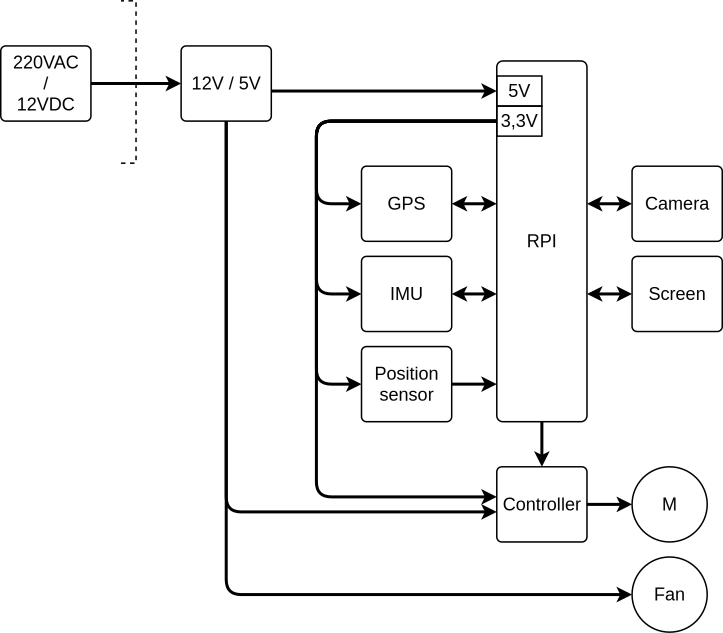
\includegraphics[width=0.7\linewidth]{\figures/sch_hardware.pdf}
    \decoRule
    \caption[
    Schéma structurel de premier niveau du télescope]{
    Schéma structurel de premier niveau du télescope}
    \label{fig:Schéma structurel de premier niveau du télescope}
    \end{figure}

\section{Conception du circuit}

\begin{figure}[H]
    \centering
    \includegraphics[width=1\linewidth]{\figures/kicad_sch2.pdf}
    \decoRule
    \caption[
    Schéma structurel de la carte du télescope]{
    Schéma structurel de la carte du télescope}
    \label{fig:Schéma structurel de la carte du télescope}
    \end{figure}

\vspace{1cm}

Ce schéma ne présente pas de subtilité particulière, la plupart des composants étant des connecteurs.

\vspace{1cm}

L'alimentation est composée de~:
\begin{itemize}[label=$\bullet$]
	\item Un interrupteur d'allumage
	\item Une diode polarisante
	\item Une diode zener protégeant des surtensions
	\item Un fusible protégeant des surintensités
	\item Un convertisseur DC/DC intégré
	\end{itemize}

\vspace{1cm}

L'environnement des boutons poussoirs servant de capteurs de butée aux mouvements du télescope est le suivant~:

\begin{figure}[H]
    \centering
    \includegraphics[width=0.3\linewidth]{\figures/sch_button.pdf}
    \decoRule
    \caption[
    Schéma de l'environnement des capteurs de butée]{
    Schéma de l'environnement des capteurs de butée}
    \label{fig:Schéma de l'environnement des capteurs de butée}
    \end{figure}

\vspace{1cm}

La valeur élevée des résistances de pullup $100k\Omega$ a pour but de réduire au maximum le courant consommé lors de l'appui, à $33\mu A$. Le courant prélevé par l'entrée GPIO de la Raspberry Pi est de l'ordre de $0,5\mu A$.

Les condensateurs de $100nF$ permettent de filtrer les parasites générés par les rebonds propres aux boutons ainsi que les perturbations électromagnétiques.

\section{Contraintes de design}

\subsection{Contraintes électromagnétiques}

La première contrainte vient de la proximité du système électronique de deux moteurs, ceux-ci générant d'importantes perturbations électromagnétiques. Cela peut être particulièrement dérangeant pour le fonctionnement de la centrale inertielle et du GPS.

La solution la plus simple et efficace est de déporter ces deux modules le long de la structure du télescope.

%\vspace{1cm}

\subsection{Contraintes mécaniques}

Ensuite viennent les contraintes mécaniques de l'association de la carte à la Raspberry Pi.

\vspace{1cm}

Tout d'abord, l'emplacement du connecteur et des fixations sont à prendre en compte.

\begin{figure}[H]
    \centering
    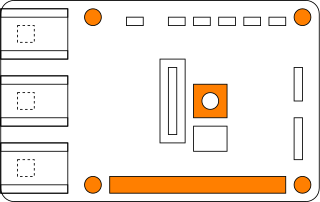
\includegraphics[width=0.5\linewidth]{\figures/sch_hard_1.pdf}
    \decoRule
    \caption[
    Schéma mécanique de la carte vue de dessus]{
    Schéma mécanique de la carte vue de dessus}
    \label{fig:Schéma mécanique de la carte vue de dessus}
    \end{figure}

\vspace{1cm}

Le connecteur d'alimentation, centré sur la carte, est un connecteur cylindrique comme ceux des ordinateurs portables. Le télescope étant amené à tourner sur lui même, ce connecteur devrait permettre le mouvement tout en empêchant le câble d'alimentation de s'emmêler ou de se détériorer.

\begin{figure}[H]
    \centering
    \includegraphics[height=0.3\linewidth]{\figures/photo_supply.jpg}
	\hspace{1cm}
    \includegraphics[height=0.3\linewidth]{\figures/photo_supply.png}
    \decoRule
    \caption[
    Connecteurs d'alimentation utilisés]{
    Connecteurs d'alimentation utilisés}
    \label{fig:Connecteurs d'alimentation utilisés}
    \end{figure}

\vspace{1cm}

Puis concernant la distance entre la carte et la Raspberry Pi, la hauteur des plus hauts éléments de la Raspberry Pi est à prendre en compte. Ainsi que la hauteur de certains condensateurs de la carte, ne pouvant donc être placés n'importe où.

\begin{figure}[H]
    \centering
    
\includegraphics[height=0.23\linewidth]{\figures/sch_hard_2.pdf}
%	\hspace{1cm}
    
\includegraphics[height=0.23\linewidth]{\figures/sch_hard_3.pdf}
    \decoRule
    \caption[
    Schéma mécanique de la carte vue de profil]{
    Schéma mécanique de la carte vue de profil}
    \label{fig:Schéma mécanique de la carte vue de profil}
    \end{figure}

\vspace{1cm}

Il faudra de plus utiliser un connecteur particulièrement haut ($16,13mm$) pour relier la carte à la Raspberry Pi.

\begin{figure}[H]
    \centering
    \includegraphics[width=0.3\linewidth]{\figures/photo_header.png}
    \decoRule
    \caption[
    Type de header utilisé]{
    Type de header utilisé}
    \label{fig:Type de header utilisé}
    \end{figure}

\section{Routage de la carte}

Le routage de la carte n'est pas terminé, voici un aperçu de son avancement actuel~:

\begin{figure}[H]
    \centering
    \includegraphics[width=0.7\linewidth]{\figures/kicad_pcb.png}
    \decoRule
    \caption[
    Aperçu du routage en cours]{
    Aperçu du routage en cours}
    \label{fig:Aperçu du routage en cours}
    \end{figure}


%\chapter{Hardware}
\label{chapter2}

\section{Choix des principaux composants}

Les principaux composants électroniques ont étés choisis en premier lieu sur les critères du prix et de la rapidité de mise en œuvre.

\vspace{1cm}

\begin{itemize}[label=$\bullet$]
	\item Le GPS : Le module adafruit-ultimate-gps (MTK3339)
	\item L'IMU : Le module Sarkfun SEN-13762 (MPU9250)
	\item Le convertisseur $12V/5V$ : Le Composant intégré Recom R-78B5.0-2.0 capable de fournir un courant de $2A$.

\section{Procédure de calibration}

Une procédure de calibration du télescope sera sans doute à prévoir à son allumage. Celle-ci ayant pour but de déterminer la direction du nord et la direction verticale.

\vspace{1cm}

À supposer que le télescope soit posé sur une surface proche de l'horizontale, la procédure consisterait~:
\begin{itemize}[label=$\bullet$]
	\item Pour l'azimut, à effectuer une rotation complète pour déterminer la direction dans laquelle le champ magnétique est le plus fort, le nord.
	\item Pour l'élévation, à balayer la plage de mouvement des croissants de la structure en observant les données de l'accéléromètre. La position dans laquelle l'accélération de la 

%\chapter{Software}
\label{chapter3}

\section{Support de la caméra}

Pour gérer les différentes configurations matérielles de façon plus "userfriendly", la Raspberry Pi dispose d'un fichier de configuration \codeinline{text}{config.txt} que le $bootloader$ interprétera pour sélectionner les $overlays$ correspondants et composer le $devicetree$ qui convient à l'architecture matérielle utilisée. Celui-ci étant ensuite passé au $kernel$ lors du démarrage.

%\vspace{1cm}

Cette subtilité propre aux Raspberry Pi permet à l'utilisateur de ne pas avoir besoin d'avoir affaire au $devicetree$ quand il s'agit de configuration. Par exemple l'activation du support d'un élément courant sur les Raspberry Pi comme le module Raspicam.

%\vspace{1cm}

le logiciel \codeinline{text}{raspi-config} n'est autre qu'une interface à ce fichier de configuration.

\vspace{1cm}

Pour activer le support matériel de la caméra, il faut ajouter les lignes suivantes à ce fichier~:

%\code{ruby}
\code{bash}
start_x=1
gpu_mem=128
\end{minted}

À travers Yocto, cela passe par l'ajout des lignes ci-dessous au fichier \codeinline{text}{local.conf} et donc à son modèle le fichier \codeinline{text}{meta-autoscope/conf/local.conf.sample} dans la $layer$ dédiée au projet.

\code{ruby}
VIDEO_CAMERA = "1"
GPU_MEM = "128"
\end{minted}

\vspace{1cm}

Quant à l'utilisation de la caméra, il existe des logiciels tels que \codeinline{text}{raspivid} pour filmer ou \codeinline{text}{raspistill} pour prendre des clichés. Tous deux font partie de la suite \codeinline{text}{userland} que l'on ajoute à notre image via la ligne ci-dessous dans le fichier\\\codeinline{text}{meta-autoscope/recipes-autoscope/images/autoscope-console-image.bb}~:

\code{ruby}
IMAGE_INSTALL += "userland"
\end{minted}

À l'usage, la commande suivante permet d'afficher en plein écran le flux vidéo jusqu'à ce qu'on le stoppe~:

\code{bash}
~$ raspivid -t 0
\end{minted}

\section{Étude de l'embarcation de Stellarium}

Une première évaluation de la faisabilité de l'embarcation de Stellarium sur la Raspberry Pi a été de l'installer via le gestionnaire de paquet sur une Raspberry Pi dotée de Raspbian.

\code{bash}
~$ sudo apt-get install stellarium
\end{minted}

\vspace{1cm}

Avec le compositeur graphique logiciel, Stellarium est totalement inutilisable. Cependant il est possible d'activer le compositeur graphique matériel. Pour cela il faut activer l'option \codeinline{text}{Advanced Options -> GL Driver} dans le menu \codeinline{text}{raspi-config}.

La différence de rendu peut être observée avec l'outil \codeinline{text}{glxgears} prévu à cet effet. Celui-ci s'installe par la ligne suivante~:

\code{bash}
~$ sudo apt-get install mesa-utils
\end{minted}

\begin{figure}[H]
    \centering
    \includegraphics[width=0.3\linewidth]{\figures/photo_glxgears.png}
    \decoRule
    \caption[
    Captures d'écran de glxgears]{
    Captures d'écran de glxgears}
    \label{fig:Captures d'écran de glxgears}
    \end{figure}

\vspace{1cm}

Le résultat est alors meilleur, Stellarium est utilisable bien qu'il lui arrive de planter lorsque l'on fait un déplacement trop brusque dans le ciel.

\vspace{1cm}

Il existe une version mobile de Stellarium disponible notament pour Android et iOS qui est une version allélégée et optimisée pour l'usage sur un smartphone.

Ses sources sont disponibles à l'adresse suivante~:\\\url{https://noctua-software.com/stellarium-mobile}

\vspace{1cm}

Il semble que cette version puisse fonctionner telle quelle sur Linux. À l'heure actuelle nous n'avons pas réussi à compiler Stellarium mobile pour un problème de dépendance à une librairie (Qt5Declarative, faisant partie du paquet qtdeclarative5-dev) qui n'existe plus dans les versions récentes de Qt, ultérieures à la version Qt5.6 pour être précis.

Le problème pourrait sans doute être résolu en récupérant ladite librairie dans les dépots d'une distribution plus ancienne, Ubuntu Xenial (Qt5.5.1) ou Trusty (Qt5.2.1) par exemple.


%\part{Clément AILLOUD}
%\chapter{Hardware}

\section{Rappel sur l'architecture de la carte}

En guise de rappel, ci-dessous un schéma de l'architecture de la carte du télescope.

\begin{figure}[H]
    \centering
    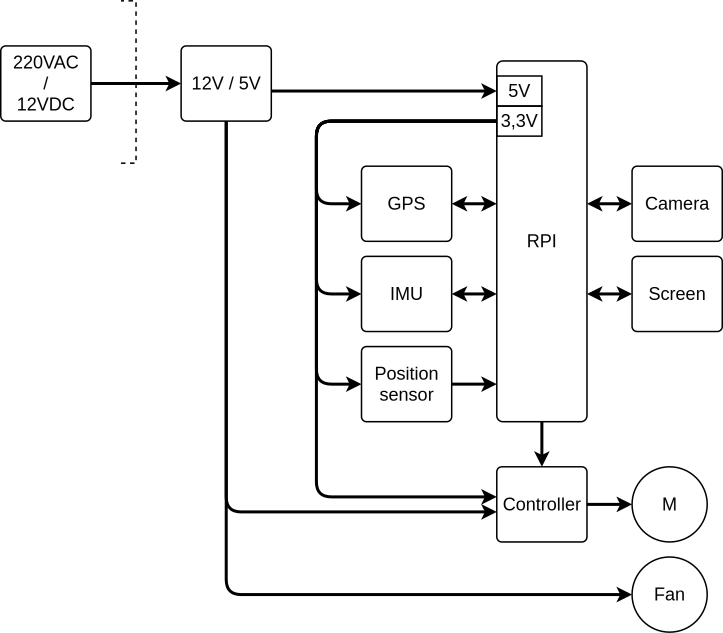
\includegraphics[width=0.7\linewidth]{\figures/sch_hardware.pdf}
    \decoRule
    \caption[
    Schéma structurel de premier niveau du télescope]{
    Schéma structurel de premier niveau du télescope}
    \label{fig:Schéma structurel de premier niveau du télescope}
    \end{figure}

\section{Conception du circuit}

\begin{figure}[H]
    \centering
    \includegraphics[width=1\linewidth]{\figures/kicad_sch2.pdf}
    \decoRule
    \caption[
    Schéma structurel de la carte du télescope]{
    Schéma structurel de la carte du télescope}
    \label{fig:Schéma structurel de la carte du télescope}
    \end{figure}

\vspace{1cm}

Ce schéma ne présente pas de subtilité particulière, la plupart des composants étant des connecteurs.

\vspace{1cm}

L'alimentation est composée de~:
\begin{itemize}[label=$\bullet$]
	\item Un interrupteur d'allumage
	\item Une diode polarisante
	\item Une diode zener protégeant des surtensions
	\item Un fusible protégeant des surintensités
	\item Un convertisseur DC/DC intégré
	\end{itemize}

\vspace{1cm}

L'environnement des boutons poussoirs servant de capteurs de butée aux mouvements du télescope est le suivant~:

\begin{figure}[H]
    \centering
    \includegraphics[width=0.3\linewidth]{\figures/sch_button.pdf}
    \decoRule
    \caption[
    Schéma de l'environnement des capteurs de butée]{
    Schéma de l'environnement des capteurs de butée}
    \label{fig:Schéma de l'environnement des capteurs de butée}
    \end{figure}

\vspace{1cm}

La valeur élevée des résistances de pullup $100k\Omega$ a pour but de réduire au maximum le courant consommé lors de l'appui, à $33\mu A$. Le courant prélevé par l'entrée GPIO de la Raspberry Pi est de l'ordre de $0,5\mu A$.

Les condensateurs de $100nF$ permettent de filtrer les parasites générés par les rebonds propres aux boutons ainsi que les perturbations électromagnétiques.

\section{Contraintes de design}

\subsection{Contraintes électromagnétiques}

La première contrainte vient de la proximité du système électronique de deux moteurs, ceux-ci générant d'importantes perturbations électromagnétiques. Cela peut être particulièrement dérangeant pour le fonctionnement de la centrale inertielle et du GPS.

La solution la plus simple et efficace est de déporter ces deux modules le long de la structure du télescope.

%\vspace{1cm}

\subsection{Contraintes mécaniques}

Ensuite viennent les contraintes mécaniques de l'association de la carte à la Raspberry Pi.

\vspace{1cm}

Tout d'abord, l'emplacement du connecteur et des fixations sont à prendre en compte.

\begin{figure}[H]
    \centering
    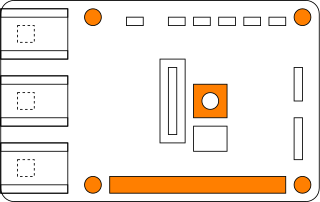
\includegraphics[width=0.5\linewidth]{\figures/sch_hard_1.pdf}
    \decoRule
    \caption[
    Schéma mécanique de la carte vue de dessus]{
    Schéma mécanique de la carte vue de dessus}
    \label{fig:Schéma mécanique de la carte vue de dessus}
    \end{figure}

\vspace{1cm}

Le connecteur d'alimentation, centré sur la carte, est un connecteur cylindrique comme ceux des ordinateurs portables. Le télescope étant amené à tourner sur lui même, ce connecteur devrait permettre le mouvement tout en empêchant le câble d'alimentation de s'emmêler ou de se détériorer.

\begin{figure}[H]
    \centering
    \includegraphics[height=0.3\linewidth]{\figures/photo_supply.jpg}
	\hspace{1cm}
    \includegraphics[height=0.3\linewidth]{\figures/photo_supply.png}
    \decoRule
    \caption[
    Connecteurs d'alimentation utilisés]{
    Connecteurs d'alimentation utilisés}
    \label{fig:Connecteurs d'alimentation utilisés}
    \end{figure}

\vspace{1cm}

Puis concernant la distance entre la carte et la Raspberry Pi, la hauteur des plus hauts éléments de la Raspberry Pi est à prendre en compte. Ainsi que la hauteur de certains condensateurs de la carte, ne pouvant donc être placés n'importe où.

\begin{figure}[H]
    \centering
    
\includegraphics[height=0.23\linewidth]{\figures/sch_hard_2.pdf}
%	\hspace{1cm}
    
\includegraphics[height=0.23\linewidth]{\figures/sch_hard_3.pdf}
    \decoRule
    \caption[
    Schéma mécanique de la carte vue de profil]{
    Schéma mécanique de la carte vue de profil}
    \label{fig:Schéma mécanique de la carte vue de profil}
    \end{figure}

\vspace{1cm}

Il faudra de plus utiliser un connecteur particulièrement haut ($16,13mm$) pour relier la carte à la Raspberry Pi.

\begin{figure}[H]
    \centering
    \includegraphics[width=0.3\linewidth]{\figures/photo_header.png}
    \decoRule
    \caption[
    Type de header utilisé]{
    Type de header utilisé}
    \label{fig:Type de header utilisé}
    \end{figure}

\section{Routage de la carte}

Le routage de la carte n'est pas terminé, voici un aperçu de son avancement actuel~:

\begin{figure}[H]
    \centering
    \includegraphics[width=0.7\linewidth]{\figures/kicad_pcb.png}
    \decoRule
    \caption[
    Aperçu du routage en cours]{
    Aperçu du routage en cours}
    \label{fig:Aperçu du routage en cours}
    \end{figure}



\appendix

%\include{Appendices/AppendixA}

\end{document}
